\chapter{Introduction}

Your work here. Cite people using either inline:~\citet{Hopkins2021213} or not:~\citep{Hopkins2021213}.
Reference figures, tables and sections like: Figure~\ref{fig:tectonic_setting}, Table:~\ref{tab:study_period_events}, Section~\ref{example}. 
Remember that all units and quantities should be separated using a non-breaking half-space: 7\,km


\section{Example figure and table}\label{example}

\begin{figure}

    \centering

    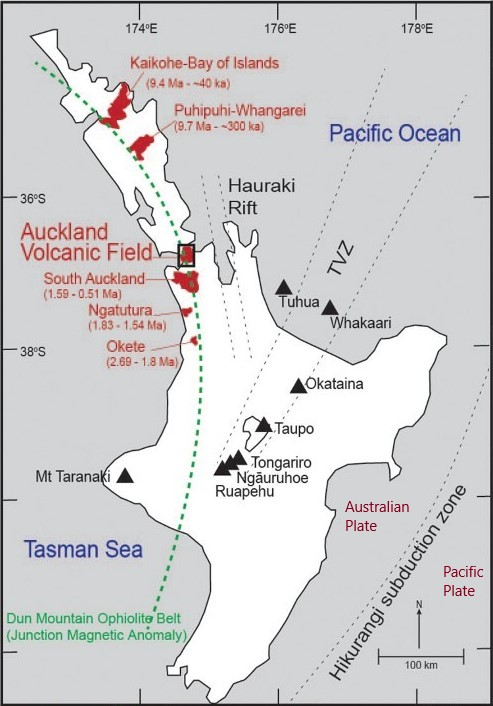
\includegraphics[width=0.9\textwidth]{./Figures/Hopkins2021Fig1Av2.jpg}

    \centering

    \caption[Short caption for ToC]{Big caption}
    \label{fig:tectonic_setting}

\end{figure}


\begin{table}
    \centering
    \caption[Short caption for ToT]{Table captions go above the table}
    \begin{tabular}{c|c|c|c|c}
        Year & Total Events & EQ & QB & Unlabelled \\
        \hline
        2011 & 45 & 13 & 32 & 0 \\
    \end{tabular}
    \label{tab:study_period_events}
\end{table}



